% \tikzset{every picture/.style={line width=0.75pt}} %set default line width to 0.75pt        

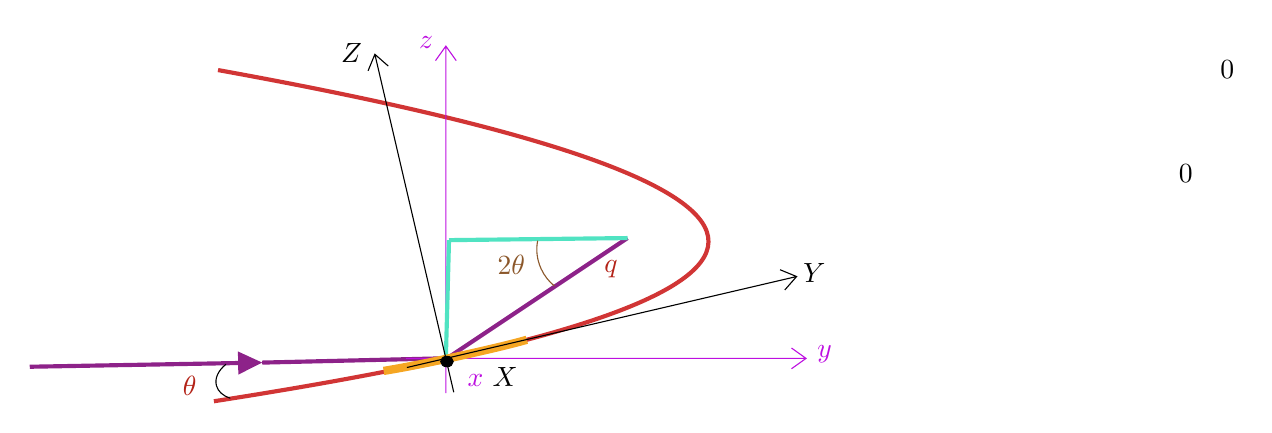
\begin{tikzpicture}[x=0.75pt,y=0.75pt,yscale=-1,xscale=1]
%uncomment if require: \path (0,214); %set diagram left start at 0, and has height of 214

%Shape: Parabola [id:dp636758281566334] 
\draw  [color={rgb, 255:red, 209; green, 53; blue, 53 }  ,draw opacity=1 ][line width=1.5]  (232.73,180.63) .. controls (549.78,131.36) and (550.44,78.17) .. (234.71,21.06) ;
%Straight Lines [id:da5751643928734858] 
\draw [color={rgb, 255:red, 141; green, 34; blue, 137 }  ,draw opacity=1 ][line width=1.5]    (256,162) -- (341,160) ;
%Straight Lines [id:da4985393188459284] 
\draw [color={rgb, 255:red, 141; green, 34; blue, 137 }  ,draw opacity=1 ][line width=1.5]    (345,160) -- (432,102) ;
%Shape: Axis 2D [id:dp5339485321600788] 
\draw [color={rgb, 255:red, 189; green, 16; blue, 224 }  ,draw opacity=1 ] (325.2,159.98) -- (518,159.98)(344.48,9.53) -- (344.48,176.7) (511,154.98) -- (518,159.98) -- (511,164.98) (339.48,16.53) -- (344.48,9.53) -- (349.48,16.53)  ;
%Straight Lines [id:da984423242776999] 
\draw [color={rgb, 255:red, 141; green, 34; blue, 137 }  ,draw opacity=1 ][line width=1.5]    (144,164) -- (252,162.07) ;
\draw [shift={(256,162)}, rotate = 538.98] [fill={rgb, 255:red, 141; green, 34; blue, 137 }  ,fill opacity=1 ][line width=0.08]  [draw opacity=0] (11.61,-5.58) -- (0,0) -- (11.61,5.58) -- cycle    ;
%Straight Lines [id:da25833218941129754] 
\draw [color={rgb, 255:red, 80; green, 227; blue, 194 }  ,draw opacity=1 ][line width=1.5]    (346,103) -- (432,102) ;
%Straight Lines [id:da4020633150416717] 
\draw [color={rgb, 255:red, 80; green, 227; blue, 194 }  ,draw opacity=1 ][line width=1.5]    (346,103) -- (344.48,159.98) ;
%Shape: Arc [id:dp507008334854385] 
\draw  [draw opacity=0] (396.83,125.12) .. controls (394.17,123.02) and (391.91,120.19) .. (390.35,116.77) .. controls (388.31,112.28) and (387.83,107.52) .. (388.71,103.28) -- (406.13,109.59) -- cycle ; \draw  [color={rgb, 255:red, 139; green, 87; blue, 42 }  ,draw opacity=1 ] (396.83,125.12) .. controls (394.17,123.02) and (391.91,120.19) .. (390.35,116.77) .. controls (388.31,112.28) and (387.83,107.52) .. (388.71,103.28) ;
%Shape: Arc [id:dp28668965321519213] 
\draw  [draw opacity=0] (240.6,179.18) .. controls (237.17,178.08) and (234.66,175.93) .. (233.92,173.03) .. controls (233.01,169.5) and (234.91,165.69) .. (238.55,162.8) -- (249.39,169.04) -- cycle ; \draw   (240.6,179.18) .. controls (237.17,178.08) and (234.66,175.93) .. (233.92,173.03) .. controls (233.01,169.5) and (234.91,165.69) .. (238.55,162.8) ;
%Curve Lines [id:da06756156046542072] 
\draw [color={rgb, 255:red, 245; green, 166; blue, 35 }  ,draw opacity=1 ][line width=3]    (314.5,166) .. controls (335.17,162.67) and (372.17,154.33) .. (383.5,151) ;
%Shape: Axis 2D [id:dp06708045637689208] 
\draw [color={rgb, 255:red, 0; green, 0; blue, 0 }  ,draw opacity=1 ] (325.7,164.37) -- (513.46,120.54)(310.28,13.46) -- (348.28,176.26) (505.5,117.26) -- (513.46,120.54) -- (507.78,127) (307,21.42) -- (310.28,13.46) -- (316.74,19.14)  ;
%Shape: Ellipse [id:dp8232202429248765] 
\draw  [fill={rgb, 255:red, 0; green, 0; blue, 0 }  ,fill opacity=1 ] (342,161.5) .. controls (342,160.12) and (343.34,159) .. (345,159) .. controls (346.66,159) and (348,160.12) .. (348,161.5) .. controls (348,162.88) and (346.66,164) .. (345,164) .. controls (343.34,164) and (342,162.88) .. (342,161.5) -- cycle ;

% Text Node
\draw (721,21) node    {$0$};
% Text Node
\draw (701,71) node    {$0$};
% Text Node
\draw (527,158) node  [color={rgb, 255:red, 179; green, 35; blue, 24 }  ,opacity=1 ,rotate=-359.63]  {$\textcolor[rgb]{0.74,0.06,0.88}{y}$};
% Text Node
\draw (335,8) node  [color={rgb, 255:red, 179; green, 35; blue, 24 }  ,opacity=1 ,rotate=-359.63]  {$\textcolor[rgb]{0.74,0.06,0.88}{z}$};
% Text Node
\draw (299,13) node  [color={rgb, 255:red, 179; green, 35; blue, 24 }  ,opacity=1 ,rotate=-359.63]  {$\textcolor[rgb]{0,0,0}{Z}$};
% Text Node
\draw (522,119) node  [color={rgb, 255:red, 179; green, 35; blue, 24 }  ,opacity=1 ,rotate=-359.63]  {$\textcolor[rgb]{0,0,0}{Y}$};
% Text Node
\draw (367,169) node  [color={rgb, 255:red, 179; green, 35; blue, 24 }  ,opacity=1 ,rotate=-359.63]  {$\textcolor[rgb]{0.74,0.06,0.88}{x} \ \textcolor[rgb]{0,0,0}{X}$};
% Text Node
\draw (424,117) node  [color={rgb, 255:red, 179; green, 35; blue, 24 }  ,opacity=1 ,rotate=-359.63]  {$q$};
% Text Node
\draw (221,173) node  [color={rgb, 255:red, 179; green, 35; blue, 24 }  ,opacity=1 ,rotate=-359.63]  {$\theta $};
% Text Node
\draw (376,115) node  [color={rgb, 255:red, 139; green, 87; blue, 42 }  ,opacity=1 ,rotate=-359.63]  {$2\theta $};


\end{tikzpicture}
